\documentclass{article}
\usepackage{float}
\usepackage{graphicx}
\usepackage[a4paper, total={6in, 8in}]{geometry}
\title{Probability and Statistics Notes}
\author{Thomas Møller Jensen}
\begin{document}
\maketitle
\section*{Lecture 1: Elementary digital circuits}
The flash converter, an analog signal can be converted from analog to digital using this converter.\ it will divide a voltage into different levels, shown as the resistors on the figure below.
This will produce a truth table of sorts, if we put in a signal that is between 2 and 3 volts in the example on the blackboard, it will correspond to the 2nd row in the table below:
\begin{figure}[H]
	\centering
	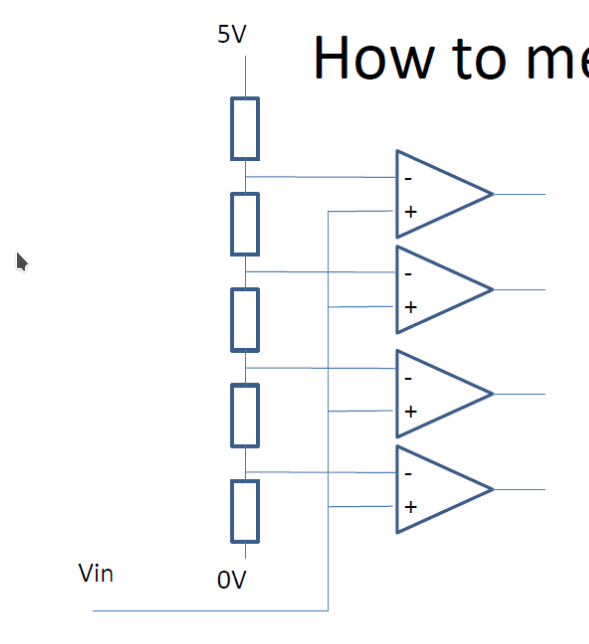
\includegraphics[width=\textwidth]{image.png}
\end{figure}
% +--------+------+
% | [0, 1) | LLLL |
% | [2, 3) | HLLL |
% | [3, 4) | HHLL |
% | [4, 5) | HHHL |
% | 5+     | HHHH |
% +--------+------+

\subsection*{Exercises}
\paragraph{1. Show by perfect induction the following relations:}

\begin{enumerate}
	\item $(A+B)*(A+C)=A+(B*C)$
	
	\begin{table}[H]
		\centering
		\begin{tabular}{|c|c|c|c|c|c|c|c|}
			\hline
			A & B & C & $A+B$ & $A+C$ & $(A+B)*(A+C)$ & $B*C$ & $A+(B*C)$ \\\hline
			0 & 0 & 0 & 0   & 0   & 0           & 0   & 0       \\\hline
			0 & 0 & 1 & 0   & 1   & 0           & 0   & 0       \\\hline
			0 & 1 & 0 & 1   & 0   & 0           & 0   & 0\\\hline
			0 & 1 & 1 & 1   & 1   & 1           & 1   & 1\\\hline
			1 & 0 & 0 & 1   & 1   & 1           & 0   & 1\\\hline
			1 & 0 & 1 & 1   & 1   & 1           & 0   & 1\\\hline
			1 & 1 & 0 & 1   & 1   & 1           & 0   & 1\\\hline
			1 & 1 & 1 & 1   & 1   & 1           & 1   & 1\\\hline
		\end{tabular}
	\end{table}
	\item $A*(A+B)=A$

	\begin{table}[H]
		\centering
		\begin{tabular}{|c|c|c|c|}
			\hline
			A & B & $A+B$ & $A*(A+B)$ \\\hline
			0 & 0 & 0   & 0       \\\hline
			0 & 1 & 1   & 0       \\\hline
			1 & 0 & 1   & 1       \\\hline
			1 & 1 & 1   & 1       \\\hline
		\end{tabular}
	\end{table}	
	\item $A+\overline{A}=1$
	
	\begin{table}[H]
		\centering
		\begin{tabular}{|c|c|c|}
			\hline
			A & $\overline{A}$ & $A+\overline{A}$ \\\hline
			0 & 1 		   & 1              \\\hline
			1 & 0 		   & 1              \\\hline
		\end{tabular}
	\end{table}	
	\item $\overline{A+B+C} = \overline{A}*\overline{B}*\overline{C}$
	
	\begin{table}[H]
		\centering
		\begin{tabular}{|c|c|c|c|c|c|c|c|c|}
			\hline
			A & B & C & $A+B+C$ & $\overline{A+B+C}$ & $\overline{A}$ & $\overline{B}$ & $\overline{C}$ & $\overline{A}*\overline{B}*\overline{C}$ \\\hline
			0 & 0 & 0 & 0     & 1                & 1            & 1            & 1   	  & 1                                      \\\hline
			0 & 0 & 1 & 1     & 0                & 1            & 1            & 0            & 0                                      \\\hline
			0 & 1 & 0 & 1     & 0                & 1            & 0            & 1            & 0                                      \\\hline
			0 & 1 & 1 & 1     & 0                & 1            & 0            & 0            & 0                                      \\\hline
			1 & 0 & 0 & 1     & 0                & 0            & 1            & 1            & 0                                      \\\hline
			1 & 0 & 1 & 1     & 0                & 0            & 1            & 0            & 0                                      \\\hline
			1 & 1 & 0 & 1     & 0                & 0            & 0            & 1            & 0                                      \\\hline
			1 & 1 & 1 & 1     & 0                & 0            & 0            & 0            & 0                                      \\\hline
		\end{tabular}
	\end{table}
\end{enumerate}

\paragraph{1. Show that the following expression is equivalent to the exclusive or function}

This is denoted by $\oplus$
\end{document}
